\section{静电场}
对应课本第三章,占分20分左右

\begin{question}
有一半径为a的导体球,原先不带电,在球外离球心为d处放一点电荷q,设导体球接地,用电像法求空间电势,球面上感应电荷密度。(要求写清楚电像法的步骤)
\end{question}

\begin{question}
在均匀外电场$E_0$中置入半径为$R_0$的导体球,导体球上带总电荷Q ,试用分离变数法求导体球外的电势。
\end{question}

\begin{question}
平行板电容器的平板间相距为d,两极间加直流电压V,
下板电势高。在下板内侧面上有一很小的半球突起,球半径为a(a=d),求电容器内的电场和半球上的电荷密度。
\begin{figure}[ht]
\centering
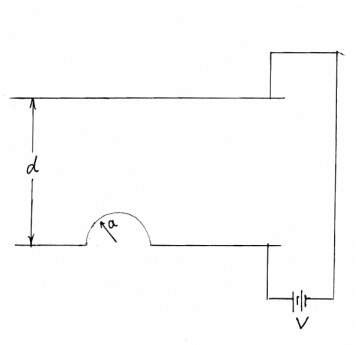
\includegraphics[height=3 cm]{images/q1_2_3.jpg}
\caption{题1.2.3}
\end{figure}

\end{question}

\begin{question}
有一半径为a的导体球,原先不带电,在球外离球心为d处放一点电荷q,设导体球接地,用电像法求空间电势,球面上感应电荷密度。(要求写清楚电像法的步骤)
\end{question}

\begin{question}
如图所示的x>0与x<0区域充满两种均匀介质,介电常数为$\varepsilon_1$与$\varepsilon_2$,在x轴上的d处有点电荷q,用电像法求空间电势。
\begin{figure}[ht]
\centering
\includegraphics[height=3 cm]{images/q1_2_5.jpg}
\caption{题1.2.5}
\end{figure}
\end{question}

\begin{question}
求真空中带电导体球的静电能量。
\end{question}

\begin{question}
有一半径为a,介电常数为$\varepsilon$的无限长电介质圆柱,柱轴沿$\textbf{\textit{e}}_z$方向
,沿$\textbf{\textit{e}}_x$方向外加一均匀电场$E_0$,求空间电势分布。
\begin{figure}[ht]
\centering
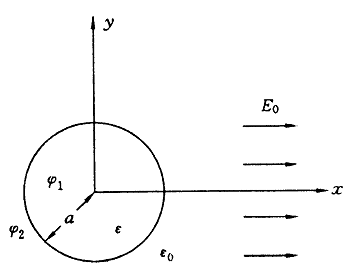
\includegraphics[height=3 cm]{images/q1_2_7.png}
\caption{题1.2.7}
\end{figure}
\end{question}

\begin{question}
一平行板电容器,板长为l,宽为b,板间距离d,如图所示,从板的左部插入一块介质,其介电常数为$\varepsilon$,插入深度为x,介质和平板之间无空隙,求介质板上受的力。略去平板电容器的边缘效应,两板间保持电位差为V。
\begin{figure}[ht]
\centering
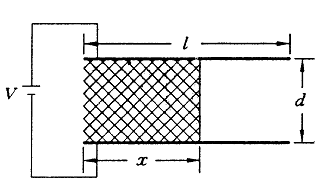
\includegraphics[height=3 cm]{images/q1_2_8.png}
\caption{题1.2.8}
\end{figure}
\end{question}

\begin{question}
如图所示 ,一半径为 a 的均匀介质球 ,介电常数为$\varepsilon_1$,介质球内带均匀自由电荷 ,电荷密度为$\rho$,介质球沉浸在介电常数为$\varepsilon_2$的无限大均匀介质中 , 在 z 方向加一均匀电场$E_0$,求球内外的电势。
\begin{figure}[ht]
\centering
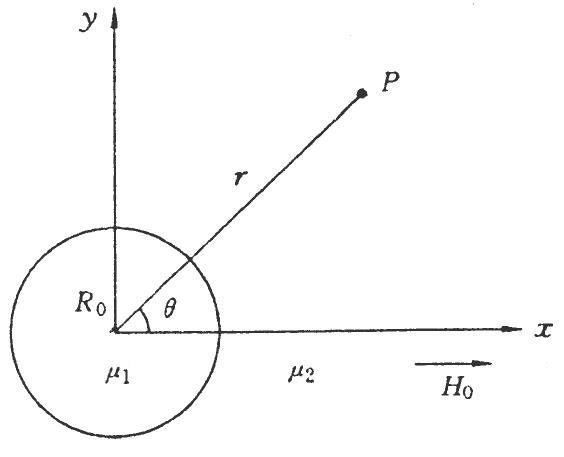
\includegraphics[height=3 cm]{images/q1_2_9.jpg}
\caption{题1.2.9}
\end{figure}
\end{question}

\begin{question}
有一均匀带电的回转椭球体 ,回转半径为a,轴半径长为c,总电量为q,计算其电偶极矩 、电四极矩以及远处的电势。
\end{question}

\begin{question}
利用格林函数方法来证明静电势的均值定理,即在无电荷的空间中的任一点的电势,等于以该点为球心任一球面上的电势的平均值。
\end{question}